%%%%%%%%%%%%%%%%%%%%%%%%%%%%%%%%
\section{Experimental Evaluation}
\label{fi:sec:experiments}

In this section, we compare LSR and I-LSR to other inference algorithms in terms of statistical efficiency and empirical performance.
First, in order to measure the statistical efficiency of the estimators, we generate synthetic data from a known ground truth.
Then, we look at five real-world datasets and investigate the practical performance of the algorithms in terms of accuracy, running time and convergence rate.

\paragraph{Error Metric}
As the probability of $i$ winning over $j$ depends on the ratio of strengths $\gamma_i / \gamma_j$, the strengths are typically logarithmically spaced.
In order to evaluate the accuracy of an estimate $\bm{\gamma}$ to ground truth parameters $\bm{\gamma}'$, we therefore use a $\log$ transformation, reminiscent of the random-utility-theoretic formulation of the choice model.
Define $\bm{\theta} \doteq [\log \gamma_i - \kappa]$, with $\kappa$ chosen such that $\sum_i \theta_i = 0$.
We will consider the root-mean-squared error
\begin{align*}
E_{\text{RMS}} = \Vert \bm{\theta} - \bm{\theta}' \Vert_2 / \sqrt{N}.
\end{align*}

\subsection{Statistical Efficiency}

To assess the statistical efficiency of LSR and other algorithms, we follow the experimental procedure of \citet{hajek2014minimax}.
We consider $N = 1024$ items, and draw $\bm{\theta}'$ uniformly at random in $[-2, 2]^N$.
We generate $M = 64$ full rankings over the $N$ items from a Plackett--Luce model parametrized with $\bm{\gamma} \propto [e^{\theta_i}]$.
For a given $K \in \{2^1, \ldots, 2^{10}\}$, we break down each of the full rankings as follows.
First, we partition the items into $N/K$ subsets of size $K$ uniformly at random.
Then, we store the $K$-way rankings induced by the full ranking on each of those subsets.
As a result, we obtain $MN/K$ statistically independent $K$-way partial rankings.
For a given estimator, this data produces an estimate $\bm{\theta}$, for which we record the root-mean-square error to $\bm{\theta}'$.
We consider four estimators.
The first two (LSR and ML) work on the ranking data directly.
The remaining two follow \citet{azari2013generalized}, who suggest breaking down $K$-way rankings into $\binom{K}{2}$ pairwise comparisons.
These comparisons are then used by LSR, resulting in \citeauthor{azari2013generalized}'s GMM-F estimator, and by an ML estimator (ML-F).
In short, the four estimators vary according to
\begin{enuminline}
\item whether they use as-is rankings or derived comparisons, and
\item whether the model is fitted using an approximate spectral algorithm or using exact maximum likelihood.
\end{enuminline}
Figure~\ref{fi:fig:efficiency} plots $E_{\text{RMS}}$ for increasing sizes of partial rankings, as well as a lower bound to the error of any estimator for the Plackett--Luce model (see \citet{hajek2014minimax} for details).
We observe that breaking the rankings into pairwise comparisons (*-F estimators) incurs a significant efficiency loss over using the $K$-way rankings directly (LSR and ML).
We conclude that by correctly weighting pairwise rates in the Markov chain, LSR distinctly outperforms the rank-breaking approach as $K$ increases.
We also observe that the MLE is always more efficient.
Spectral estimators such as LSR provide a computationally inexpensive, asymptotically consistent estimate of parameters, but this observation justifies calling them \emph{approximate} inference algorithms.


\begin{figure}
\centering
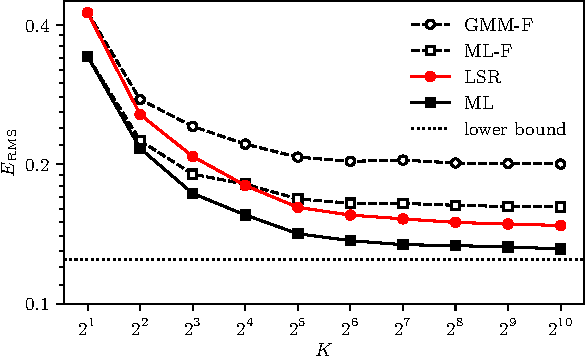
\includegraphics{fi-efficiency}
\caption{
Statistical efficiency of different estimators for increasing sizes of partial rankings.
As $K$ grows, breaking rankings into pairwise comparisons becomes increasingly inefficient.
LSR remains efficient at no additional computational cost.
}
\label{fi:fig:efficiency}
\end{figure}

\subsection{Empirical Performance}

We investigate the performance of various inference algorithms on five real-world datasets.
The NASCAR \citep{hunter2004mm} and sushi \citep{kamishima2009efficient} datasets contain multiway partial rankings.
The YouTube\footnote{%
See: \url{https://archive.ics.uci.edu/ml/machine-learning-databases/00223/}.},
GIFGIF\footnote{%
See: \url{http://lucas.maystre.ch/gifgif-data}.}
and chess\footnote{%
See: \url{https://www.kaggle.com/c/chess}.}
datasets contain pairwise comparisons.
Among those, the chess dataset is particular in that it features 45\% of ties;
in this case we use the model proposed by \citet{rao1967ties}.
We preprocess each dataset by discarding items that are not part of the largest strongly connected component in the comparison graph, in order to ensure that the MLE is well-defined.
For each  dataset, the number of items $N$, the number of rankings $M$, as well as the size $K$ of a partial ranking after preprocessing are given in Table~\ref{fi:tab:approxalg}.

\paragraph{Experimental Procedure}
All experiments are run on a machine with a quad-core 2.0 GHz Haswell processor and 16 GB of RAM, running Mac OS X 10.9.
For LSR and I-LSR, we use a slightly adapted version the Python code presented in Listing~\ref{fi:lst:implementation}, which calls a dense LU factorization routine.
We implement the Rank Centrality (RC), GMM-F and MM \citep{hunter2004mm} algorithms in Python as well.
For the Newton-Raphson algorithm, we implement the choice model on top of the popular \texttt{statsmodels} Python library\footnote{%
See: \url{http://statsmodels.sourceforge.net/}
} that provides a Newton-Raphson solver.
We have compared our implementation of the MM algorithm to that of \citeauthor{hunter2004mm} written in Matlab\footnote{%
See: \url{http://sites.stat.psu.edu/~dhunter/code/btmatlab/}
}, and observed that ours has comparable running time.
For the chess dataset, we use the Rao--Kupper model with $\alpha = \sqrt{2}$ for simplicity.
Note that this parameter could also be estimated from the data, however in our experiments we focus on the performance of algorithms for estimating $\bm{\gamma}$.

\begin{lstlisting}[
  caption={Python implementation of one iteration of I-LSR.},
  label={fi:lst:implementation},
  language=Python,
  numbers=none,
  frame=single]
import numpy as np
import scipy.linalg as spl

def weighted_lsr(n, rankings, weights):
    chain = np.zeros((n, n), dtype=float)
    for ranking in rankings:
        sum_weights = sum(weights[x] for x in ranking)
        for i, winner in enumerate(ranking):
            val = 1.0 / sum_weights
            for loser in ranking[i+1:]:
                chain[loser, winner] += val
            sum_weights -= weights[winner]
    chain -= np.diag(chain.sum(axis=1))
    return statdist(chain)

def statdist(chain):
    lu, piv = spl.lu_factor(generator.T)
    res = spl.solve_triangular(lu[:-1,:-1], -lu[:-1,-1])
    res = np.append(res, 1.0)
    return res / res.sum()
\end{lstlisting}

We first compare the estimates produced by three approximate ML inference algorithms, LSR, GMM-F and RC.
Note that RC applies only to pairwise comparisons, and that LSR is the only algorithm able to infer the parameters in the Rao-Kupper model.
Also note that in the case of pairwise comparisons, GMM-F and LSR are strictly equivalent.
In Table~\ref{fi:tab:approxalg}, we report the root-mean-square deviation to the MLE $\bm{\theta}^\star$ and the running time $T$ of the algorithm.

\sisetup{group-minimum-digits=4,detect-weight=true}
\begin{table}[ht]
  \caption{Performance of approximate ML inference algorithms.}
  \label{fi:tab:approxalg}
  \centering
  \small{
  \begin{tabular}{l rrr rr rr rr rr}
    \toprule
            &             &               &          & \multicolumn{2}{c}{LSR}            & \multicolumn{2}{c}{GMM-F}          & \multicolumn{2}{c}{RC} \\
                                                       \cmidrule(l){5-6}                    \cmidrule(l){7-8}                    \cmidrule(l){9-10}
    Dataset &         $N$ &           $M$ &      $K$ &     $E_{\text{RMS}}$ &     $T$ [s] &     $E_{\text{RMS}}$ &     $T$ [s] & $E_{\text{RMS}}$ & $T$ [s] \\
    \midrule
    NASCAR  &    \num{83} &      \num{36} & \num{43} & \bfseries\num{0.194} &  \num{0.03} &          \num{0.751} &  \num{0.06} &         --- &         --- \\
    Sushi   &   \num{100} &    \num{5000} & \num{10} & \bfseries\num{0.034} &  \num{0.22} &          \num{0.130} &  \num{0.19} &         --- &         --- \\
    \addlinespace                                                                                                             
    YouTube & \num{16187} & \num{1128704} &  \num{2} & \bfseries\num{0.417} & \num{34.18} & \bfseries\num{0.417} & \num{34.18} & \num{0.432} & \num{41.91} \\
    GIFGIF  &  \num{5503} &   \num{95281} &  \num{2} & \bfseries\num{1.286} &  \num{1.90} & \bfseries\num{1.286} &  \num{1.90} & \num{1.295} &  \num{2.84} \\
    \addlinespace                                                                                                             
    Chess   &  \num{6174} &   \num{63421} &  \num{2} & \bfseries\num{0.420} &  \num{2.90} &                  --- &         --- &         --- &         --- \\
    \bottomrule
  \end{tabular}
  }
\end{table}

The smallest value of $E_{\text{RMS}}$ is highlighted in bold for each dataset.
We observe that in the case of multiway partial rankings, LSR is almost four times more accurate than GMM-F on the datasets considered.
In the case of pairwise comparisons, RC is slightly worse than LSR and GMM-F, because the number of comparisons per pair is not homogeneous (see Section~\ref{fi:sec:pairwise}).
The running time of the three algorithms is comparable.

Next, we turn our attention to ML inference and consider three iterative algorithms: I-LSR, MM and Newton-Raphson.
For Newton-Raphson, we use an off-the-shelf solver.
Each algorithm is initialized with $\bm{\gamma}^{(0)} = [1/N \  \cdots \  1/N]^\Tr$, and convergence is declared when $E_{\text{RMS}} < 0.01$.
In Table~\ref{fi:tab:mlalg}, we report the number of iterations $I$ needed to reach convergence, as well as the total running time $T$ of the algorithm.

\begin{table}[ht]
  \caption{Performance of iterative ML inference algorithms.}
  %The algorithms are stopped when the estimate has a RMSE $< 0.01$.}
  \label{fi:tab:mlalg}
  \centering
  \small{
  \begin{tabular}{l r rr rr rr}
    \toprule
             &             & \multicolumn{2}{c}{I-LSR}        & \multicolumn{2}{c}{MM}      & \multicolumn{2}{c}{Newton} \\
                             \cmidrule(l){3-4}                  \cmidrule(l){5-6}             \cmidrule(l){7-8}
    Dataset  & $\xi$               & $I$ &         $T$ [s] &        $I$ &        $T$ [s] &     $I$ &     $T$ [s] \\
    \midrule
    NASCAR   & \num{0.832} &  \num{3} &   \bfseries\num{0.08} &    \num{4} &     \num{0.10} &     --- &         --- \\
    Sushi    & \num{0.899} &  \num{2} &   \bfseries\num{0.42} &    \num{4} &     \num{1.09} & \num{3} & \num{10.45} \\
    \addlinespace
    YouTube  & \num{0.002} & \num{12} & \bfseries\num{414.44} & \num{8680} & \num{22443.88} &     --- &         --- \\
    GIFGIF   & \num{0.408} & \num{10} &  \bfseries\num{22.31} &  \num{119} &   \num{109.62} & \num{5} & \num{72.38} \\
    \addlinespace
    Chess    & \num{0.007} & \num{15} &  \bfseries\num{43.69} &  \num{181} &    \num{55.61} & \num{3} & \num{49.37} \\
    \bottomrule
  \end{tabular}
  }
\end{table}

The smallest total running time $T$ is highlighted in bold for each dataset.
We observe that Newton-Raphson does not always converge, despite the log-likelihood being strictly concave\footnote{
On the NASCAR dataset, this has also been noted by \citet{hunter2004mm}.
Computing the Newton step appears to be severely ill-conditioned for many real-world datasets.
We believe that it can be addressed by a careful choice of starting point, step size, or by monitoring the numerical stability;
however, these modifications are non-trivial and impose an additional burden on the practitioner.
}.
I-LSR consistently outperforms MM and Newton-Raphson in running time.
Even if the average running time per iteration is in general larger than that of MM, it needs considerably fewer iterations:
For the YouTube dataset, I-LSR yields an increase in speed of over $50$ times.

The slow convergence of minorization-maximization algorithms is known \citep{hunter2004mm}, yet the scale of the issue and its apparent unpredictability is surprising.
In Hunter's MM algorithm, updating a given $\gamma_i$ involves only parameters of items to which $i$ has been compared.
Therefore, we speculate that the convergence rate of MM is dependent on the expansion properties of the comparison graph $\mathcal{G}_{\mathcal{D}}$.
As an illustration, we consider the sushi dataset.
To quantify the expansion properties, we look at the spectral gap $\xi$ of a simple random walk on $\mathcal{G}_{\mathcal{D}}$;
intuitively, the larger the spectral gap is, the better the expansion properties are \citep{levin2008markov}.
The original comparison graph is almost complete, and $\xi = 0.899$.
By breaking each \num{10}-way ranking into \num{5} independent pairwise comparisons, we effectively sparsify the comparison graph.
As a result, the spectral gap decreases to \num{0.815}.
In Figure~\ref{fi:fig:convergence}, we show the convergence rate of MM and I-LSR for the original ($K = 10$) and modified ($K = 2$) datasets.
We observe that both algorithms display linear convergence, however the rate at which MM converges appears to be sensitive to the structure of the comparison graph.
In contrast, I-LSR is robust to changes in the structure.
The spectral gap of each dataset is listed in Table~\ref{fi:tab:mlalg}.
%Therefore, to better interpret the result of Table~\ref{fi:tab:mlalg}, we also list for each dataset the spectral gap of its comparison graph.


\begin{figure}
\centering
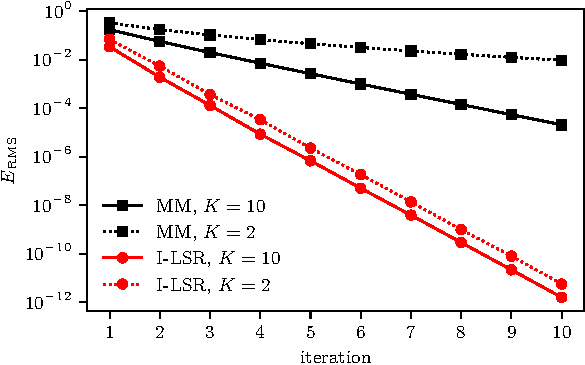
\includegraphics{fi-convergence}
\caption{
Convergence rate of I-LSR and MM on the sushi dataset.
When partial rankings ($K = 10$) are broken down into independent comparisons ($K = 2$), the comparison graph becomes sparser.
I-LSR is robust to this change, whereas the convergence rate of MM significantly decreases.
}
\label{fi:fig:convergence}
\end{figure}

